\documentclass[9pt]{beamer} 
\usetheme{cwc} 

\usepackage{amsmath,amssymb}
\usepackage{graphicx,acronym,setspace,epstopdf,IEEEtrantools}
\usepackage[ruled]{algorithm2e}
\usepackage{subeqnarray,multirow,cite,array,color,mathtools,setspace,geometry}

\let\oldfootnote\footnote
\renewcommand\footnote[1][]{\oldfootnote[frame,#1]}

\acrodef{MSE}{mean squared error}
\acrodef{BC}{broadcast channel}
\acrodef{MC}{multi-cell}
\acrodef{BS}{base station}
\acrodef{MIMO}{multiple-input multiple-output}
\acrodef{SISO}{single-input single-output}
\acrodef{MU}{multi-user}
\acrodef{MU-MIMO}{\acl{MU} \acl{MIMO}}
\acrodef{OFDM}{orthogonal frequency division multiplexing}
\acrodef{WSRM}{weighted sum rate maximization}
\acrodef{QoS}{quality of service}
\acrodef{SCA}{successive convex approximation}
\acrodef{SNR}{signal-to-noise ratio}
\acrodef{MMSE}{minimum \acl{MSE}}
\acrodef{SIR}{signal-to-interference ratio}
\acrodef{SINR}{signal-to-interference-plus-noise ratio}
\acrodef{Q-WSRM}{queue \acl{WSRM}}
\acrodef{QM}{queue minimizing}
\acrodef{SRA}{spatial resource allocation}
\acrodef{JSFRA}{joint space-frequency resource allocation}
\acrodef{WMMSE}{weighted \acl{MMSE}}
\acrodef{KKT}{Karush-Kuhn-Tucker}
\acrodef{GP}{geometric programming}
\acrodef{SOC}{second-order cone}
\acrodef{BCDM}{block coordinate descent method}
\acrodef{BiT}{Bi-directional training}

\newcommand{\mbf}[1]{\mathbf{#1}}
\newcommand{\me}[1]{\( #1 \)}
\newcommand{\mc}[1]{\mathcal{#1}}
\newcommand{\fall}{\forall}
\newcommand{\set}[1]{\left \lbrace #1 \right \rbrace }
\newcommand{\mvec}[2]{\mathbf{#1}_{#2}}
\newcommand{\ith}[1]{{#1}^\mathrm{th}}
\newcommand{\pr}[1]{{#1}^\prime}
\newcommand{\mbfa}[1]{{\boldsymbol{#1}}}
\newcommand{\herm}{\mathrm{H}}
\newcommand{\sset}[1]{\left [ #1 \right ]}
\newcommand{\rfrac}[2]{{}^{#1}/{}_{#2}}
\newcommand{\eqspace}{\IEEEeqnarraynumspace}
\newcommand{\enoise}{\widetilde{N}_0}
\newcommand{\eqsub}{\IEEEyessubnumber}
\newcommand{\eqsubn}{\IEEEyesnumber \IEEEyessubnumber*}
\newcommand{\neqsub}{\IEEEnosubnumber}
\newcommand{\review}[1]{{\textcolor[rgb]{0 0 0.6}{#1}}}
\newcommand{\trace}{\mathrm{tr}}
\newcommand{\tran}{\mathrm{T}}
\newcommand{\R}[1]{\label{#1}\linelabel{#1}}
\newcommand{\lr}[1]{page~\pageref{#1}, line~\lineref{#1}}
\newcommand{\eqn}[1]{\(#1\)}
\newcommand{\mx}{\mbf{m}}
\newcommand{\my}{\mbf{w}}
\newcommand{\mz}{\mbfa{\gamma}}
\newcommand{\mxb}{{{\mbf{m}}}}
\newcommand{\myb}{{{\mbf{w}}}}
\newcommand{\iterate}[2]{{#1}^{(#2)}}
\newcommand{\iter}[3]{{#1}_{#2}^{(#3)}}
\newcommand{\ma}{\mbf{x}}
\acrodef{MSE}{mean squared error}
\acrodef{IBC}{interference broadcast channel}
\acrodef{MC}{multi-cell}
\acrodef{BS}{base station}
\acrodef{MIMO}{multiple-input multiple-output}
\acrodef{SISO}{single-input single-output}
\acrodef{MU}{multiple-users}
\acrodef{OFDM}{orthogonal frequency division multiplexing}
\acrodef{WSRM}{weighted sum rate maximization}
\acrodef{QoS}{quality of service}
\acrodef{SCA}{successive convex approximation}
\acrodef{SNR}{signal-to-noise ratio}
\acrodef{MMSE}{minimum \acl{MSE}}
\acrodef{SIR}{signal-to-interference ratio}
\acrodef{SINR}{signal-to-interference-plus-noise ratio}
\acrodef{Q-WSRM}{queue \acl{WSRM}}
\acrodef{QM}{queue minimizing}
\acrodef{SRA}{spatial resource allocation}
\acrodef{JSFRA}{joint space-frequency resource allocation}
\acrodef{WMMSE}{weighted \acl{MMSE}}
\acrodef{KKT}{Karush-Kuhn-Tucker}
\acrodef{GP}{geometric programming}
\acrodef{SOC}{second-order cone}
\acrodef{BCDM}{block coordinate descent method}
\acrodef{ADMM}{alternating directions method of multipliers}
\acrodef{PD}{primal decomposition}
\acrodef{DD}{dual decomposition}
\acrodef{FFR}{fractional frequency reuse}
\acrodef{DC}{difference of convex}
\acrodef{Q-WSRME}{\ac{Q-WSRM} extended}

\graphicspath{{./}{./../Figures/}{./../Figures/Linux/}{./../Figures/Review/}{./../../flaming-octo-dangerzone/TeX3/Figures/}}
\DeclareGraphicsExtensions{.eps}

\epstopdfsetup{update,prepend,prefersuffix=false,suffix=}
\DeclareGraphicsRule{.eps}{pdf}{.pdf}{`epstopdf #1}
\pdfcompresslevel=9

\linespread{1.4}

\title{Traffic Aware Precoder Design for Space Frequency Resource Allocation}

\author{{Ganesh Venkatraman\eqn{^\dagger}, Antti T\"{o}lli, Le-Nam Tran and Markku Juntti} \\ \scriptsize{Email: \{gvenkatr, antti.tolli, le.nam.tran, markku.juntti\}@ee.oulu.fi}}


\begin{document}

\AtBeginSection{\frame{\sectionpage}}

\begin{frame}
    \titlepage
\end{frame}

\begin{frame}{Outline} \scriptsize
    \tableofcontents
\end{frame}

\acused{BS} \acused{MIMO} \acused{OFDM}

\section{Introduction}

\begin{frame}{Introduction and Motivation}
\begin{itemize}
\item Complex algorithms are adopted to maximize throughput to satisfy the data requirements from higher layers
\item Available wireless resources are to be utilized efficiently to minimize the backlogged packets 
\item Spatial and Frequency resources are exploited to empty the packets waiting at the \acp{BS}
\item We discuss precoder designs for \acl{MU} \acs{MIMO}-\acs{OFDM} setup to minimize the number of queued packets 
\end{itemize}
\end{frame}

\section{System Model \& Problem Formulation}

\begin{frame}{Symbols used}
\begin{itemize}
\item \acs{OFDM} system with \me{N} sub-channels and \me{N_B} \acp{BS}, each equipped with \me{N_T} transmit antennas
\item Let \me{K} be the total number of users with \me{N_R} antennas
\item Let \me{\mc{B}} and \me{\mc{U}} denote the set of coordinating \acp{BS} and users in the system
\item Let \me{L} be the total available spatial streams for a user \me{k}, given by \me{\min (N_T,N_R)}
\end{itemize}
\end{frame}

\begin{frame}{System Model}
\begin{itemize}
\item The \me{\ith{l}} spatial signal received on sub-channel \me{n} of user \me{k} is given by
\begin{multline}\label{eqn-1}
\hat{d}_{l,k,n} = \mvec{w}{l,k,n}^\herm \mvec{H}{b_k,k,n} \,\mvec{m}{l,k,n} d_{l,k,n} + \mvec{w}{l,k,n}^\herm \mvec{n}{l,k,n} \\ 
+ \mvec{w}{l,k,n}^\herm \sum_{i \in \mc{U} \backslash \set{k}} \mvec{H}{b_i,k,n} \sum_{j = 1}^L \mvec{m}{j,i,n}d_{j,i,n}
\end{multline}
\item where \me{\mvec{m}{l,k,n}} and \me{\mvec{w}{l,k,n}} are transmit and receive beamformers corresponding to the \me{\ith{l}} spatial stream on the \me{\ith{n}} sub-channel of user \me{k}
\end{itemize}
\end{frame}

\begin{frame}{System Model}
\begin{itemize}
\item \me{\mvec{H}{b_k,k,n} \in \mathbb{C}^{N_R \times N_T}} denotes the channel between \ac{BS} \me{b_k} and user \me{k}
\item \me{d_{l,k,n}} and \me{{n}_{l,k,n}} correspond to data symbol and equivalent noise on \me{\ith{l}} spatial stream of user \me{k}
\item Using the above notations, the \acs{SINR} seen by the \me{\ith{l}} spatial stream on the \me{\ith{n}} sub-channel for user \me{k} is given by
\end{itemize}
\begin{equation}\label{eq:SINR}
\gamma_{l,k,n} = \dfrac{\left |\mvec{w}{l,k,n}^\herm \, \mvec{H}{b_k,k,n} \, \mvec{m}{l,k,n} \right |^2}{\enoise + \sum_{(j,i) \neq (l,k)} |\mvec{w}{l,k,n}^\herm \mvec{H}{b_i,k,n} \mvec{m}{j,i,n} |^2}
\end{equation}
\begin{itemize}
\item where \eqn{\enoise = \|\mvec{w}{l,k,n}^\herm \mvec{n}{l,k,n} \|^2 }
\end{itemize}
\end{frame}

\begin{frame}{System Model with User Queues}
	\begin{figure}
		\centering
		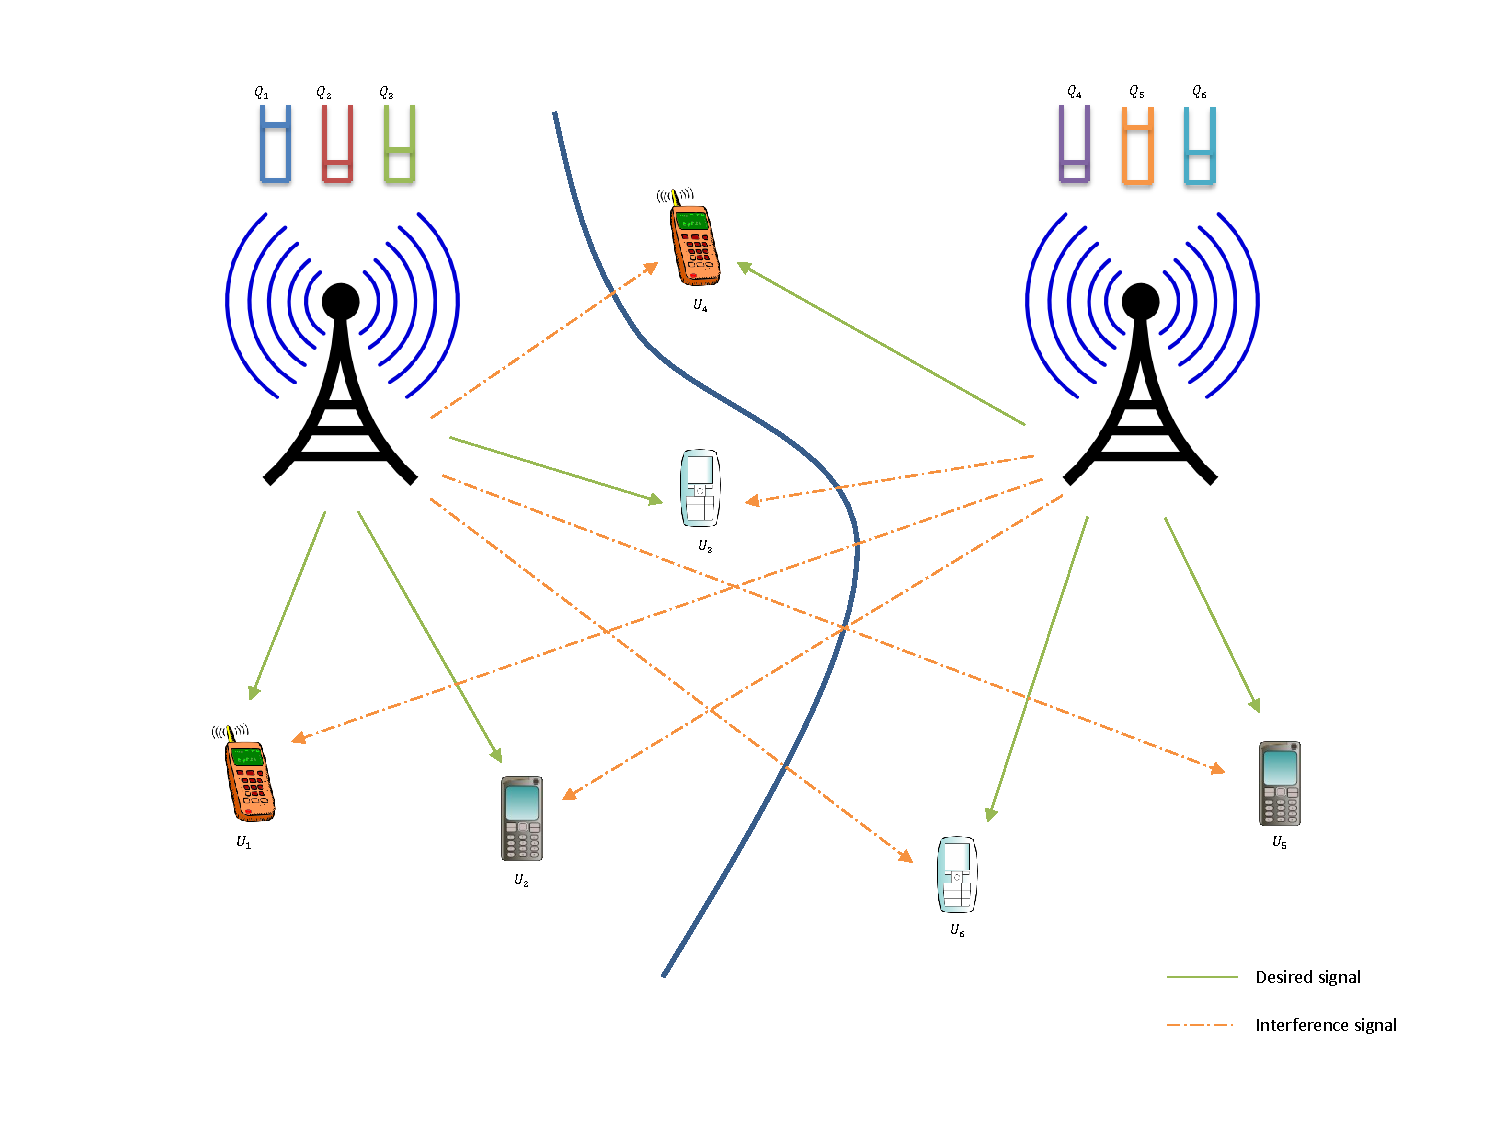
\includegraphics[width=0.9\columnwidth]{system-scenario.pdf}
	\end{figure}
\end{frame}

\begin{frame}{Queueing Model}
\begin{itemize}
\item Each user is associated with backlogged packets of size \me{Q_k} packets.
\item Queued packets \me{Q_k} of each user follows dynamic equation at the \me{\ith{i}} instant as
\begin{equation}
Q_k(i+1) = \Big [ Q_k(i) - t_k(i) \Big ]^+ + \lambda_k(i)
\label{eqn-2a}
\end{equation}
\item where \me{t_k = \sum_{n = 1}^N \, \sum_{l = 1}^L \, t_{l,k,n}} denotes the total number of transmitted packets corresponding to user \me{k} in the previous \me{\ith{i}} instant
\item \me{\lambda_k} represents the fresh arrivals of user \me{k} at \ac{BS} \me{b_k}
\end{itemize}
\end{frame}

\begin{frame}{Problem Formulation}
\begin{itemize}
\item {\color{red}Objective} - to minimize the number of backlogged packets waiting at \acp{BS}
\item {\color{red}Optimization variables} - transmit precoders and receive beamformers
\item {\color{red}\ac{MIMO}-\ac{OFDM}} - scheduling of users across sub-channels is inherently performed by precoders
\end{itemize}
\end{frame}

\section{Centralized Solutions}

\subsection{Existing \acs{Q-WSRM} Formulation}

\begin{frame}{Queue-Weighted Sum Rate Maximization (\acs{Q-WSRM})}
\begin{itemize}
\item \acs{Q-WSRM} formulation is the result of \textcolor{blue}{minimizing the conditional Lyapunov drift}\footnote{Neely, Michael J. "Stochastic network optimization with application to communication and queueing systems." Synthesis Lectures on Communication Networks 3.1 (2010): 1-211.}
\item \acs{Q-WSRM} formulation is also called as \alert{back pressure algorithm}, since it acts greedily in minimizing the backlogged packets at each instant
\[ \underset{t_{l,k,n}}{\text{minimize}} \quad \sum_{k \in \mc{U}} \left \lbrace Q_k(i)^2 - Q_k(i-1)^2 \right \rbrace, \]
\item where \me{Q_k} follows the dynamic Queue expression in \eqref{eqn-2a}
\end{itemize}
\end{frame}

\begin{frame}{Queue-Weighted Sum Rate Maximization (\acs{Q-WSRM})}
\begin{itemize}
\item \acs{Q-WSRM} formulation, which is obtained by solving Lyapunov drift, is given by
\end{itemize}
\begin{subequations}
\begin{align}
 \underset{t_{l,k,n}}{\text{maximize}} & \qquad \sum_{k \in \mc{U}} \; Q_k \left ( \alert{\sum_{n=1}^N} \, \sum_{l = 1}^L  t_{l,k,n} \right ) \\
& \qquad {\color{blue} \alert{\sum_{n=1}^N} \, \sum_{l = 1}^L  t_{l,k,n}  \leq \alert{Q_k} \; / \; Q_{k,n}}
\end{align}
\end{subequations}
\begin{itemize}
\item Queue-Rate product is maximized
\item Users with more number of backlogged packets are favored over good channel users
\end{itemize}
\end{frame}

\subsection{\acs{JSFRA} Formulation (\acs{SINR} Relaxation)}

\begin{frame}{\acs{JSFRA} Formulation (\acs{SINR} Relaxation)}
\begin{itemize}
\item Centralized Design - precoders are designed by a controller, which are then used by all \acp{BS} in \me{\mc{B}}
\item The objective used to design transmit precoders is 
\begin{equation}
\scriptsize {\color{blue} v_k = \left | Q_k - \sum_{n = 1}^N \sum_{l = 1}^{L} t_{l,k,n} \right |^q }
\end{equation}
\item To generalize the objective, we use \me{\tilde{v}_k \triangleq a_k^{\frac{1}{q}} \, v_k}, where \me{a_k} is arbitrary weights used control the priorities
\item Exponent \me{q} plays different role based on the value it assumes
	\begin{itemize}
	\item \me{\ell_{q=1}} \alert{results in greedy allocation}
	\item \me{\ell_{q=2}} \alert{ideal for the delay or buffer size limited scenarios}
	\item \me{\ell_{q=\infty}} \alert{provides fair resource allocation in each transmission instant}
	\end{itemize}
\end{itemize}
\end{frame}

\begin{frame}{\acs{JSFRA} Formulation (\acs{SINR} Relaxation)}
\begin{itemize}
\item Optimization problem with queue difference objective is nonconvex due to the constraint
\begin{subequations}  \scriptsize
\begin{align}
\underset{\mvec{m}{l,k,n}}{\text{minimize}} & \qquad \left | Q_k - \sum_{n = 1}^N \sum_{l = 1}^{L} \log \left (1 + \gamma_{l,k,n} \right) \right |^q \\
\text{subject to} & \qquad \alert{\gamma_{l,k,n} \leq \dfrac{\left |\mvec{w}{l,k,n}^H \, \mvec{H}{b_k,k,n} \, \mvec{m}{l,k,n} \right |}{\beta_{l,k,n}}^2 } \\
& \qquad \enoise + \sum_{(j,i) \neq (l,k)} |\mvec{w}{l,k,n}^\herm \mvec{H}{b_i,k,n} \mvec{m}{j,i,n} |^2 \leq \beta_{l,k,n}
\end{align}
\end{subequations}
\item The nonconvex constraints are approximated by sequence of convex subsets and solved iteratively by \alert{\ac{SCA} method}
\item Receive beamformers are designed by the \acs{MMSE} receivers using the converged transmit precoders
\end{itemize}
\end{frame}

\subsection{\acs{JSFRA} Formulation (\acs{MSE} Reformulation)}

\begin{frame}{\acs{JSFRA} Formulation (\acs{MSE} Reformulation)}
	\begin{itemize}
	\item Alternatively, we solve the queue minimization problem by utilizing the relation between the \acs{MSE} and the \acs{SINR} as 
	\begin{eqnarray}
	\color{blue} \epsilon_{l,k,n} = (1 + \gamma_{l,k,n})^{-1}
	\end{eqnarray}
	\item Equivalence is valid only when the receivers are designed with the \ac{MSE} objective, \textit{i.e.}, \textcolor{blue}{using \acs{MMSE} receivers}
	\item Problem involves nonconvex constraint 
	\begin{subeqnarray}
	\color{red}{t_{l,k,n}} &\alert{\leq}& \alert{-\log_2(\epsilon_{l,k,n})} \\
	\epsilon_{l,k,n} &=& \mathbb{E} \big [ ( d_{l,k,n} - \hat{d}_{l,k,n} )^2 \big ] = \big | 1 - \mvec{w}{l,k,n}^\herm \mvec{H}{b_k,k,n} \mvec{m}{l,k,n} \big |^2 \nonumber \\
	&\quad& + \sum_{{(j,i) \neq (l,k)}} \big | \mvec{w}{l,k,n}^\herm \mvec{H}{b_i,k,n} \mvec{m}{j,i,n} \big |^2 + \enoise
	\end{subeqnarray}
	\end{itemize}
\end{frame}

\begin{frame}{\acs{JSFRA} Formulation (\acs{MSE} Reformulation)}
	\begin{itemize}
		\item The nonconvex constraint is approximated by a sequence of convex constraints, which is performed using \ac{SCA} technique
		\item The iterative procedure is carried out until convergence or for suitable number of iterations
		\item \alert{The above reformulation works only with the \acs{MMSE} receiver}
	\end{itemize}
\end{frame}

\subsection{Simulation Results}

\begin{frame}{Centralized Solutions}
	\begin{figure}
		\centering
		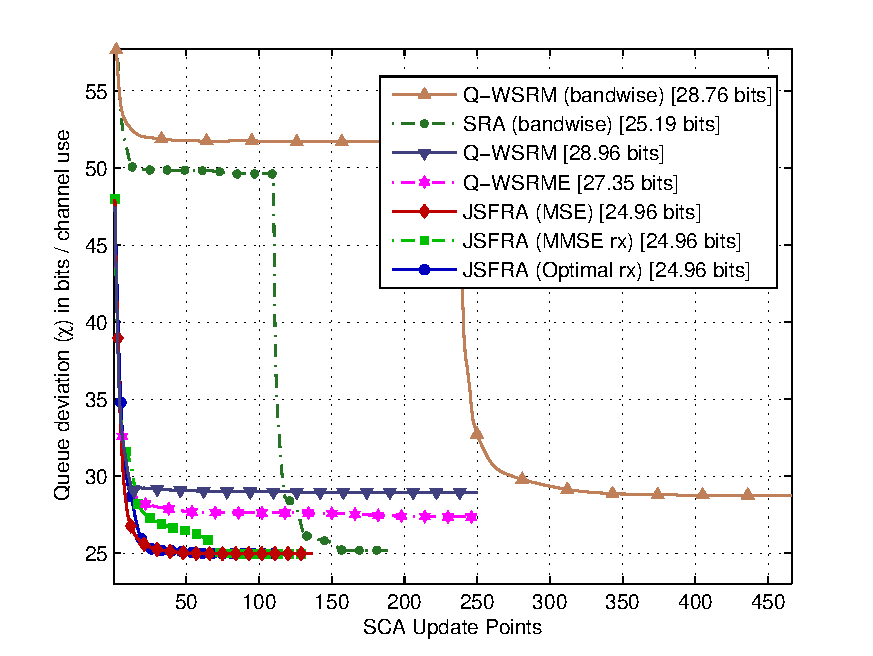
\includegraphics[width=0.75\textwidth]{fig-2-5}
		\caption{System Model - \me{\lbrace N,N_B,K,N_T,N_R \rbrace = \lbrace 2,3,9,4,2\rbrace}}
	\end{figure}
\end{frame}

\begin{frame}{Time Correlated Fading - Centralized Performance}
	\begin{figure}
		\centering
		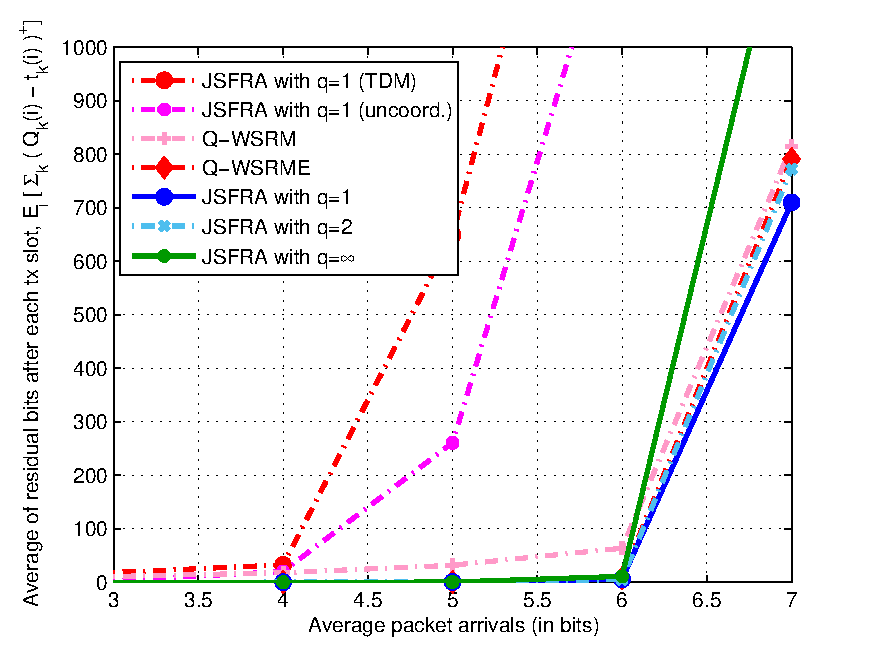
\includegraphics[width=0.75\textwidth]{average_queue_over_time-3}
		\caption{System Model - \me{\lbrace N,N_B,K,N_R \rbrace = \lbrace 3,2,8,1 \rbrace} after \eqn{250} transmissions}
	\end{figure}
\end{frame}

\section{Distributed Solutions}

\subsection{Primal \& \acs{ADMM} based decompositions}

\begin{frame}{Distributed Methods}
	\begin{itemize}
		\item \alert{Small System - centralized approach is viable}, provided channel remains constant for multiple transmission slots
		\item However, overhead involved in the centralized design scales up significantly as the network size grows
		\item Distributed approaches based on primal decomposition or \acs{ADMM} can be used to reduce the signaling requirements
		\item Signaling involved in the design of precoders are only \alert{scalar interference variables}
		\item Approximated convex subproblem in each \acs{SCA} step is performed via distributed methods
	\end{itemize}
\end{frame}

\begin{frame}{Primal Decomposition Method}
	\begin{itemize}
		\item Precoder design is based on master-slave approach
		\item Interference to the neighboring \ac{BS} users are \alert{bounded by a scalar variable, treated as a constant in subproblems}
		\item The interference thresholds are determined by the master problem and used in each slave subproblem constraint as
		\begin{equation} \label{inter_exp} \scriptsize
		\zeta_{l,k,n,b} \geq \sum_{i \in \mc{U}_b} \sum_{j = 1}^L |\mvec{w}{l,k,n}^\herm \mvec{H}{b,k,n} \mvec{m}{j,i,n} |^2 \; \forall b \in \bar{\mc{B}}_{b_k}.
		\end{equation}
	\end{itemize}
\end{frame}

\acused{ADMM}
\begin{frame}{ADMM based Decomposition Method}
	\begin{itemize}
		\item The \ac{ADMM} is superior to other distributed schemes in terms of the convergence speed
		\item \ac{ADMM} includes an additional quadratic term 
		\begin{equation}
		\color{blue} \|v_k\|_q + \sum_{l,k,n} \nu_{l,k,n}^{(j)} \left ( \mbfa{\zeta}_b - \mbfa{\zeta}^{(j)}_b \right ) + \frac{\rho}{2}  \| \mbfa{\zeta}_b - \mbfa{\zeta}^{(j)}_b \|^2
		\end{equation}
		in objective, where \eqn{\mbfa{\zeta}^{(j)}_b} is global consensus variable
		\item \eqn{\zeta_{l,k,n,b}} in \eqref{inter_exp} is \alert{treated as an optimization variable in \ac{ADMM}}
		\item Consensus variables are updated upon exchanging corresponding local \eqn{\zeta_{l,k,n,b}}'s among coordinating \acp{BS}
	\end{itemize}
\end{frame}

\subsection{KKT based Distributed Solution}

\begin{frame}{KKT based Distributed Solution}
	\begin{itemize}
		\item Decentralization methods involve significant signaling exchanges via backhaul
		\item \alert{Overhead is large for multi-antenna receivers} - iterative design should reduce the backlogged packets significantly in first few iterations
		\item To achieve that, we design precoders by solving the \ac{KKT} equations of the \acs{JSFRA} problem via \acs{MSE} reformulation
		\item \alert{Group update of all involved optimization variables} - to speed up the convergence of precoder design
	\end{itemize}
\end{frame}

\subsection{Simulation Results}

\begin{frame}{Performance of Distributed Solutions}
	\begin{figure}
		\centering
		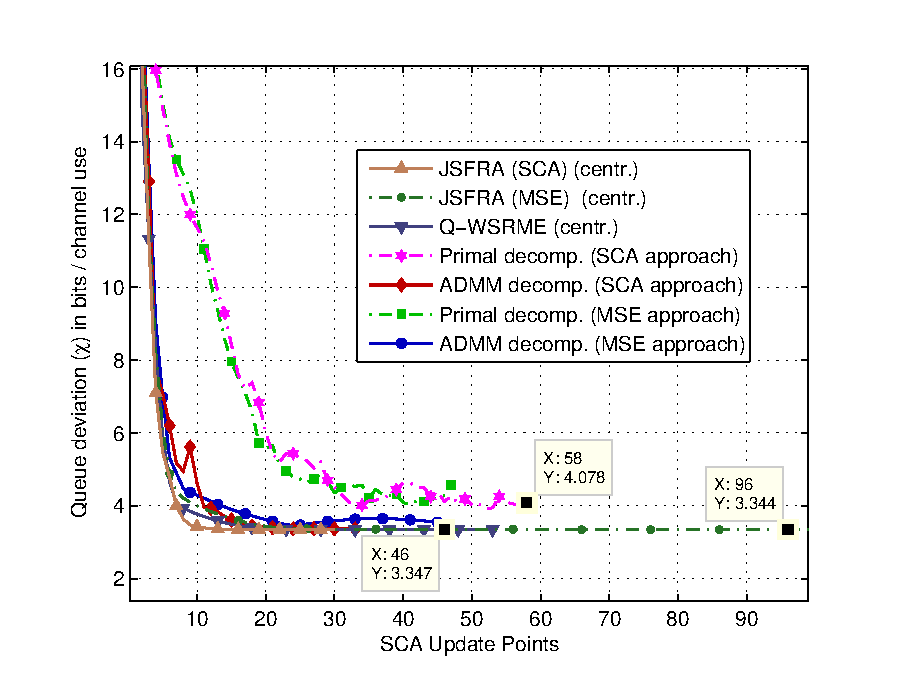
\includegraphics[width=0.75\textwidth]{fig-3-2}
		\caption{System Model - \me{\lbrace N,N_B,K,N_T,N_R \rbrace = \lbrace 3,2,8,4,1 \rbrace}}
	\end{figure}
\end{frame}

\begin{frame}{Performance of KKT based Approach}
	\begin{figure}
		\centering
		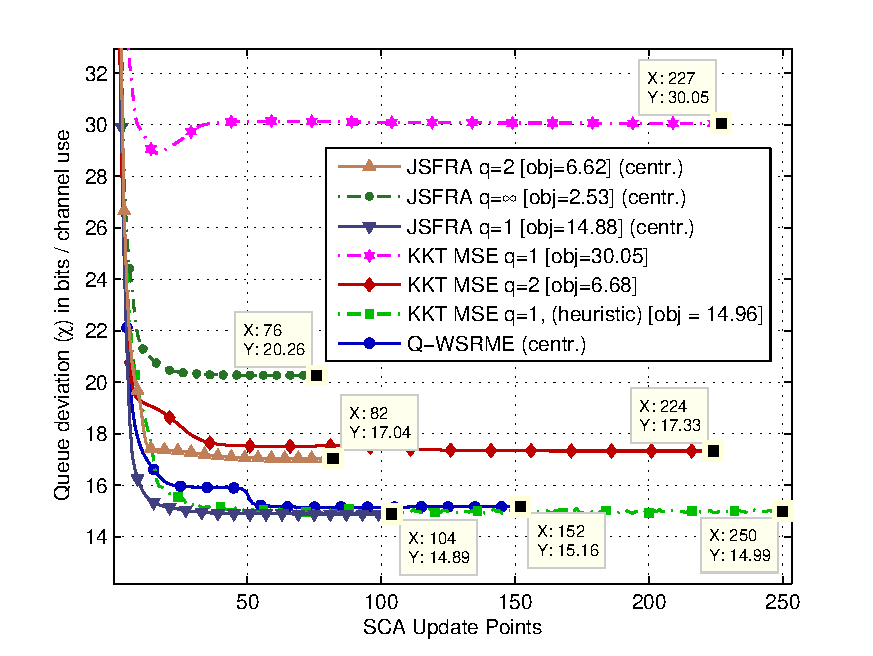
\includegraphics[width=0.75\textwidth]{fig-9-3}
		\caption{System Model - \me{\lbrace N,N_B,K,N_T,N_R \rbrace = \lbrace 5,2,8,4,1 \rbrace}}
	\end{figure}
\end{frame}

\section{Time Correlated Fading Performance}

\subsection{Methods to Update Precoders via \acs{OTA}}

\begin{frame}{Time Correlated Precoder Design - Introduction}
	\begin{itemize}
		\item So far, we have discussed few methods to design precoders in a distributed manner
		\item Now, we discuss a \textcolor{red}{practical approach to design precoders with minimal backhaul usage}
		\item To discuss further, we consider \ac{KKT} based design for following reasons
		\begin{itemize}
			\item Due to closed form solution, \textcolor[rgb]{0,0.6,0}{each \ac{SCA} update requires only single exchange of coupling variables}
			\item Moreover, transmit and receive precoders expressions can be formed by using precoded pilot transmissions
		\end{itemize}
		\item We \textcolor[rgb]{0,0,0.6}{adopt \ac{BiT}} to update transmit and receive beamformers \footnote{P. Komulainen, A. T\"olli \& M. Juntti, “Effective CSI Signaling and Decentralized Beam Coordination in TDD Multi-Cell MIMO Systems”, IEEE Transactions on Signal Processing, vol. 61, no. 9, pp. 2204 -- 2218, May 2013}
	\end{itemize}	
\end{frame}

\begin{frame}{Time Correlated Precoder Design - Strategy A}
	\begin{itemize}
		\item To devise \ac{OTA} based iterative algorithm - let us consider transmit and receive beamformer expressions
		\begin{IEEEeqnarray*}{ll}
		\mvec{m}{l,k,n}^{(i)} &= \Big (\displaystyle \sum_{x \in \mc{U}} \sum_{y=1}^L \alpha_{y,x,n}^{(i-1)} \mvec{H}{b_k,x,n}^\herm \mvec{w}{y,x,n}^{(i-1)} \mvec{w}{y,x,n}^{\herm \, {(i-1)}} \mvec{H}{b_k,x,n} + \delta_b \mbf{I}_{N_T} \Big )^{-1} \alpha^{(i-1)}_{l,k,n} \mvec{H}{b_k,k,n}^\herm \mvec{w}{l,k,n}^{(i-1)}  \\
		\mvec{w}{l,k,n}^{(i)} &= \Big (\displaystyle \sum_{x\in\mc{U}}\sum_{y=1}^L \mvec{H}{b_x,k,n} \mvec{m}{y,x,n}^{(i)} \mvec{m}{y,x,n}^{\herm \, (i)} \mvec{H}{b_{x},k,n}^\herm + N_0 \mathbf{I}_{N_R} \Big ) ^{-1} \; \mvec{H}{b_k,k,n} \; \mvec{m}{l,k,n}^{(i)}
		\end{IEEEeqnarray*}
		\item Note that transmit precoders \eqn{\mvec{m}{l,k,n}} depend on \eqn{\mvec{H}{b_k,i,n}^\tran \mvec{u}{l,i,n}}, \textit{i.e.}, \textcolor{blue}{effective uplink channel}
		\item Similarly, receive beamformers \eqn{\mvec{w}{l,k,n}} depend on \eqn{\mvec{H}{b_k,i,n} \mvec{m}{l,k,n}}, \textit{i.e.}, \textcolor[rgb]{0,0.6,0}{effective downlink channel}
	\end{itemize}	
\end{frame}

\begin{frame}{Time Correlated Precoder Design - Strategy A}
	\begin{itemize}
		\item To update receive beamformers at the user terminals, \textcolor{blue}{each \ac{BS} transmits precoded downlink pilots orthogonally} by using \eqn{\mvec{m}{l,k,n}^{(i)}}
		\item Upon receiving effective channel, each user update the respective receive beamformer
		\item Similarly, to update transmit beamformers at \acp{BS}, \textcolor[rgb]{0,0.6,0}{each user transmits two precoded pilot transmission}, namely, \eqn{\sqrt{\alpha_{l,k,n}^{(i-1)}} \mvec{w}{l,k,n}^\ast} and \eqn{\alpha_{l,k,n} \mvec{w}{l,k,n}^{\ast}}
		\item Upon receiving two uplink precoded pilots, each \ac{BS} then evaluates the respective transmit beamformers of all users
		\item The above iterative procedure is performed until convergence or for predetermined number of updates - \alert{Strategy A}
	\end{itemize}	
\end{frame}

\begin{frame}{Bi-directional Frame Structure}
	\begin{itemize}
		\item To perform iterative \ac{OTA} based update, we \textcolor[rgb]{0.7,0,0}{consider \ac{TDD} frame format}
		\item Using \ac{OTA} transmissions, \textcolor[rgb]{0,0.6,0}{effective channel can be conveyed to \acp{BS} and users by precoded pilots}
	\end{itemize}
	\begin{figure}
		\centering
		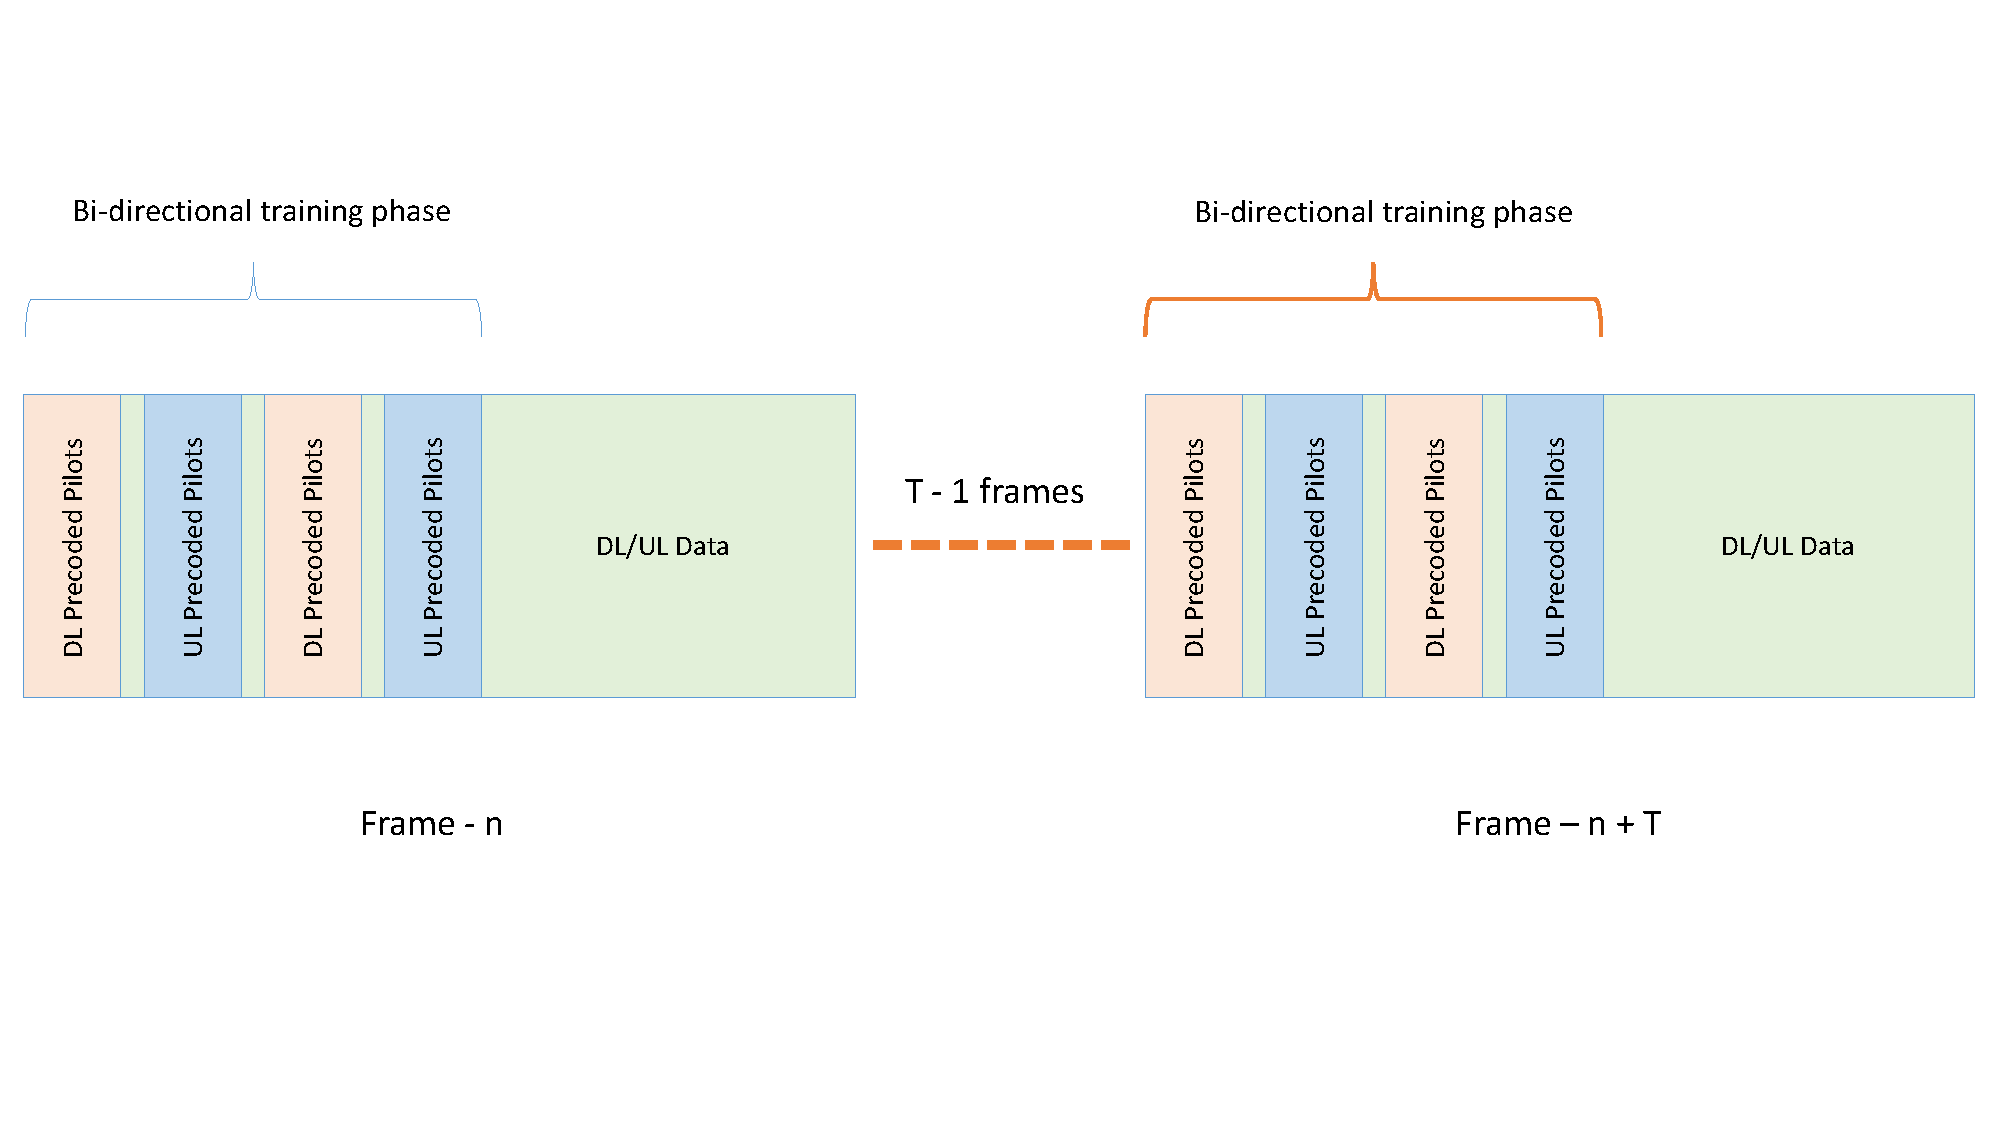
\includegraphics[trim=4mm 40mm 10mm 10mm,clip, width=\columnwidth ]{bit_model.pdf}
		\label{fig-a}
	\end{figure}
\end{frame}

\begin{frame}{Time Correlated Precoder Design - Strategy B}
	\begin{itemize}
		\item To \alert{speed up the convergence} of iterative algorithm, we update the precoders of desired users \textcolor[rgb]{0,0.6,0}{locally by fixing neighboring \acp{BS} transmit beamformers}
		\item To do so, in addition to the signaling requirements in strategy A, \textcolor[rgb]{0,0,0.6}{inter-cell interference covariance seen by desired users} is also fed back to serving \ac{BS}, \textit{i.e.},
		\begin{equation}
		\mvec{Z}{l,k,n} = \sum_{i \in \mc{U} \backslash \mc{U}_b} \mvec{H}{b_i,i,n} \mvec{m}{l,i,n} \mvec{m}{l,i,n}^\herm \mvec{H}{b_i,i,n}^\herm + N_0 \mbf{I}_{N_R}.
		\end{equation}
		\item Since inter-cell interference covariance is not required explicitly, \textcolor[rgb]{0.6,0,0}{effective whitened channel is enough to evaluate precoders}
		\item The whitening filter \eqn{\mvec{Q}{l,k,n}} is given by \eqn{\mvec{Z}{l,k,n}^{-1} = \mvec{Q}{l,k,n}^\herm \mvec{Q}{l,k,n}}
		\item Whitened channel is constructed at \ac{BS} by \textcolor[rgb]{0,0.6,0}{transmitting columns of \eqn{\mvec{Q}{l,k,n}} orthogonally from each user}
	\end{itemize}	
\end{frame}

\begin{frame}{Time Correlated Precoder Design - Strategy B}
	\begin{itemize}
		\item Upon receiving \eqn{\mvec{Q}{l,k,n}}, \textcolor[rgb]{0,0.6,0}{each \ac{BS} can construct whitened channel} as \eqn{\mvec{\bar{H}}{b_k,k} = \mvec{Q}{l,k,n} \mvec{H}{b_k,k}}
		\item The \ac{BS} specific local iteration \eqn{j} to update transmit and receive beamformer is given as
	\end{itemize}	
\begin{IEEEeqnarray*}{ll} \label{kkt-mse-x} \neqsub
	\mvec{m}{l,k,n}^{(j)} =& \Big ( \sum_{x \in \mc{U}_b} \sum_{y=1}^L \alpha_{y,x,n}^{(j-1)} \mvec{\bar{H}}{b_k,x,n}^\herm \mvec{w}{y,x,n}^{(j-1)} \mvec{w}{y,x,n}^{\herm \, {(j-1)}} \mvec{\bar{H}}{b_k,x,n} + \delta_b \mbf{I}_{N_T} \Big )^{-1} \alpha^{(j-1)}_{l,k,n} \mvec{\bar{H}}{b_k,k,n}^\herm \mvec{w}{l,k,n}^{(j-1)} \\
	\mvec{w}{l,k,n}^{(j)} =& \Big ( \sum_{x\in\mc{U}_b}\sum_{y=1}^L \mvec{\bar{H}}{b_x,k,n} \mvec{m}{y,x,n}^{(j)} \mvec{m}{y,x,n}^{\herm \, (j)} \mvec{\bar{H}}{b_{x},k,n}^\herm + \mathbf{I}_{N_R} \Big ) ^{-1} \; \mvec{\bar{H}}{b_k,k,n} \; \mvec{m}{l,k,n}^{(j)} 
\end{IEEEeqnarray*}
\begin{itemize}
	\item The above iterative procedure is performed until convergence or for predetermined number of updates - \alert{Strategy B}
\end{itemize}
\end{frame}


\begin{frame}{Summary - Signaling Requirement for OTA based Updates}
\begin{figure}
	\centering
	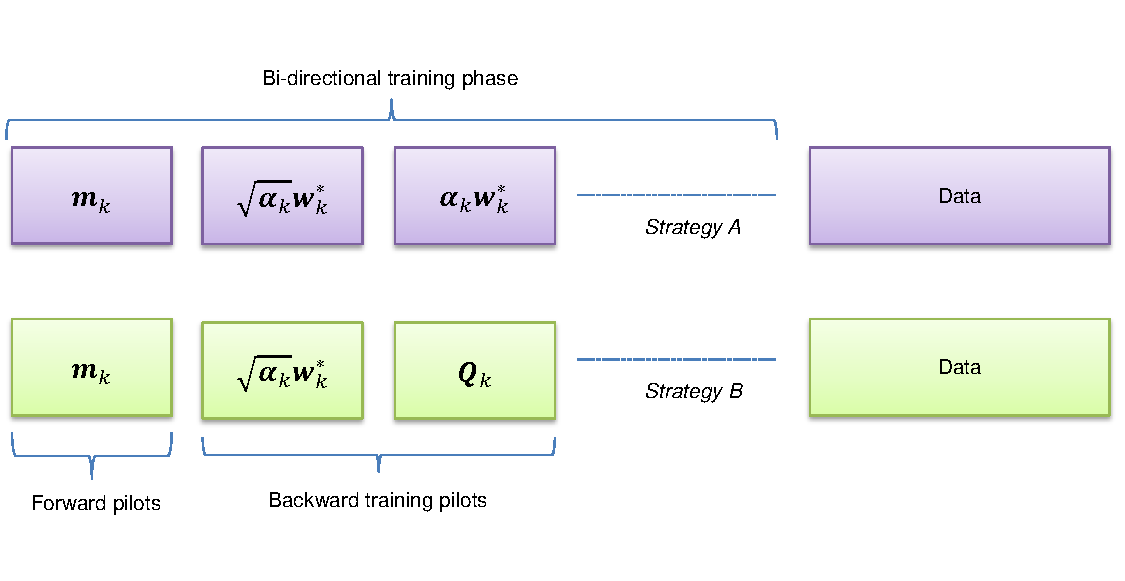
\includegraphics[trim=0mm 10mm 0mm 10mm, width=\columnwidth ]{Doc2.pdf}
	\caption{\ac{TDD} frame structure with \ac{BiT} signaling}
	\label{fig-a}
\end{figure}
\end{frame}

\subsection{Simulation Results}

\begin{frame}{Assumptions and Evaluation Model}
	\begin{itemize}
		\item Every \ac{BS} and user terminal uses \textcolor[rgb]{0,0.6,0}{orthogonal pilots in UL and DL \ac{OTA} signaling}
		\item For simplicity, pilot transmissions used to convey the equivalent channel information in one \ac{BiT} iteration - \textcolor[rgb]{0,0,0.6}{consume \eqn{\eta} resource share}.\footnote{In practice, the performance depends on the amount of available pilots and the size of coherence block.}
		\item Under this assumption, the effective rate by considering the signaling overhead is given as
		\begin{equation} \label{penalty}
		\tilde{t}_{l,k,n} = \left ( 1 - I_{\max} \, \eta \right ) \times t_{l,k,n}
		\end{equation}
		\item Total number of backlogged packets is evaluated as - \eqn{\textstyle \chi = \sum_{k = 1}^K \; [ Q_k - \tilde{t}_k ]^+}
		\item In all simulations, \textcolor[rgb]{0.6,0,0}{we consider \eqn{\eta = 1 \%}}
	\end{itemize}	
\end{frame}

\begin{frame}{Average Backlogged Packets - Distributed Design}
	\begin{figure}
		\centering
		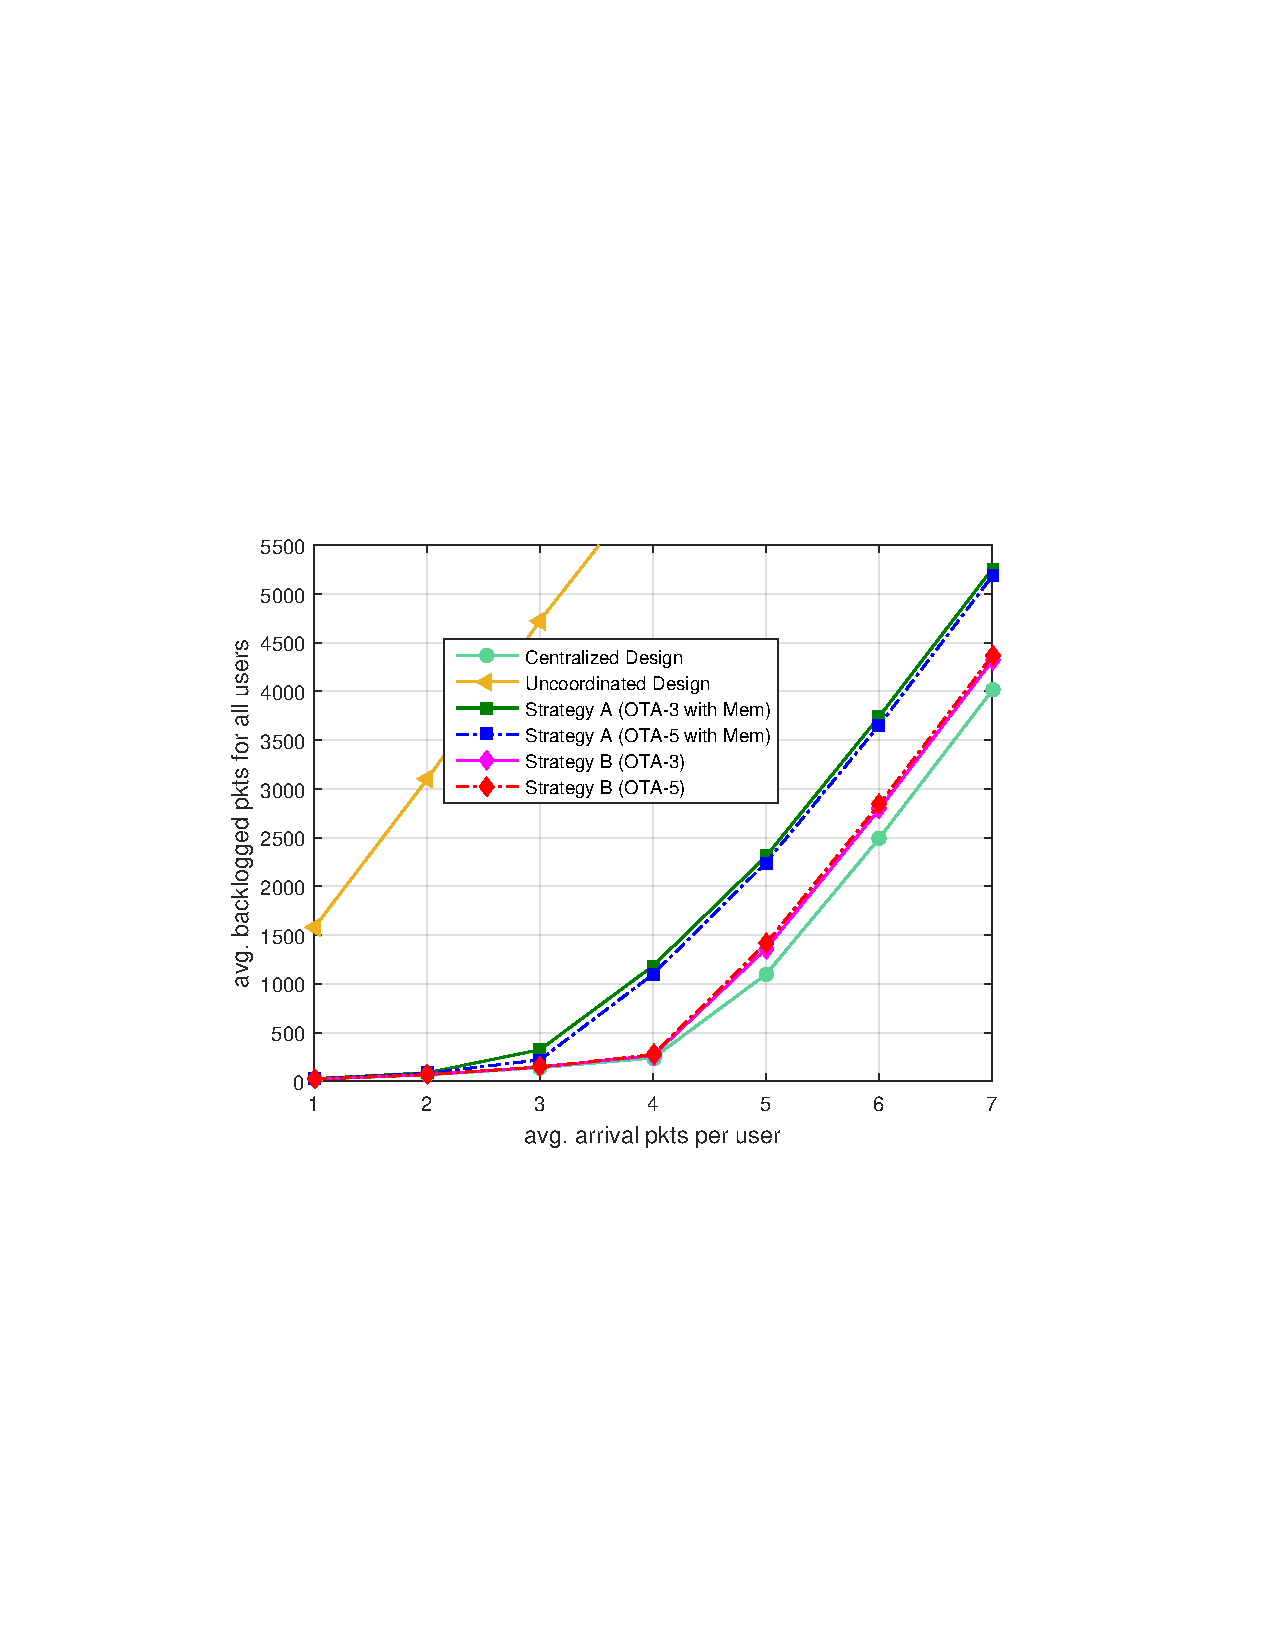
\includegraphics[trim=5mm 90mm 5mm 90mm,clip, width=\columnwidth]{ICC-A-B-1}
		\caption{Average backlogged packets for \eqn{\lbrace N,N_B,K,N_T,N_R \rbrace = \lbrace 3,2,12,4,2 \rbrace} evaluated over \eqn{250} slots with \eqn{f_dT_s\approx 0.1}}
		\label{fig-1}
	\end{figure}
\end{frame}


\begin{frame}{Average Backlogged Packets - Distributed Design}
	\begin{figure}
		\centering
		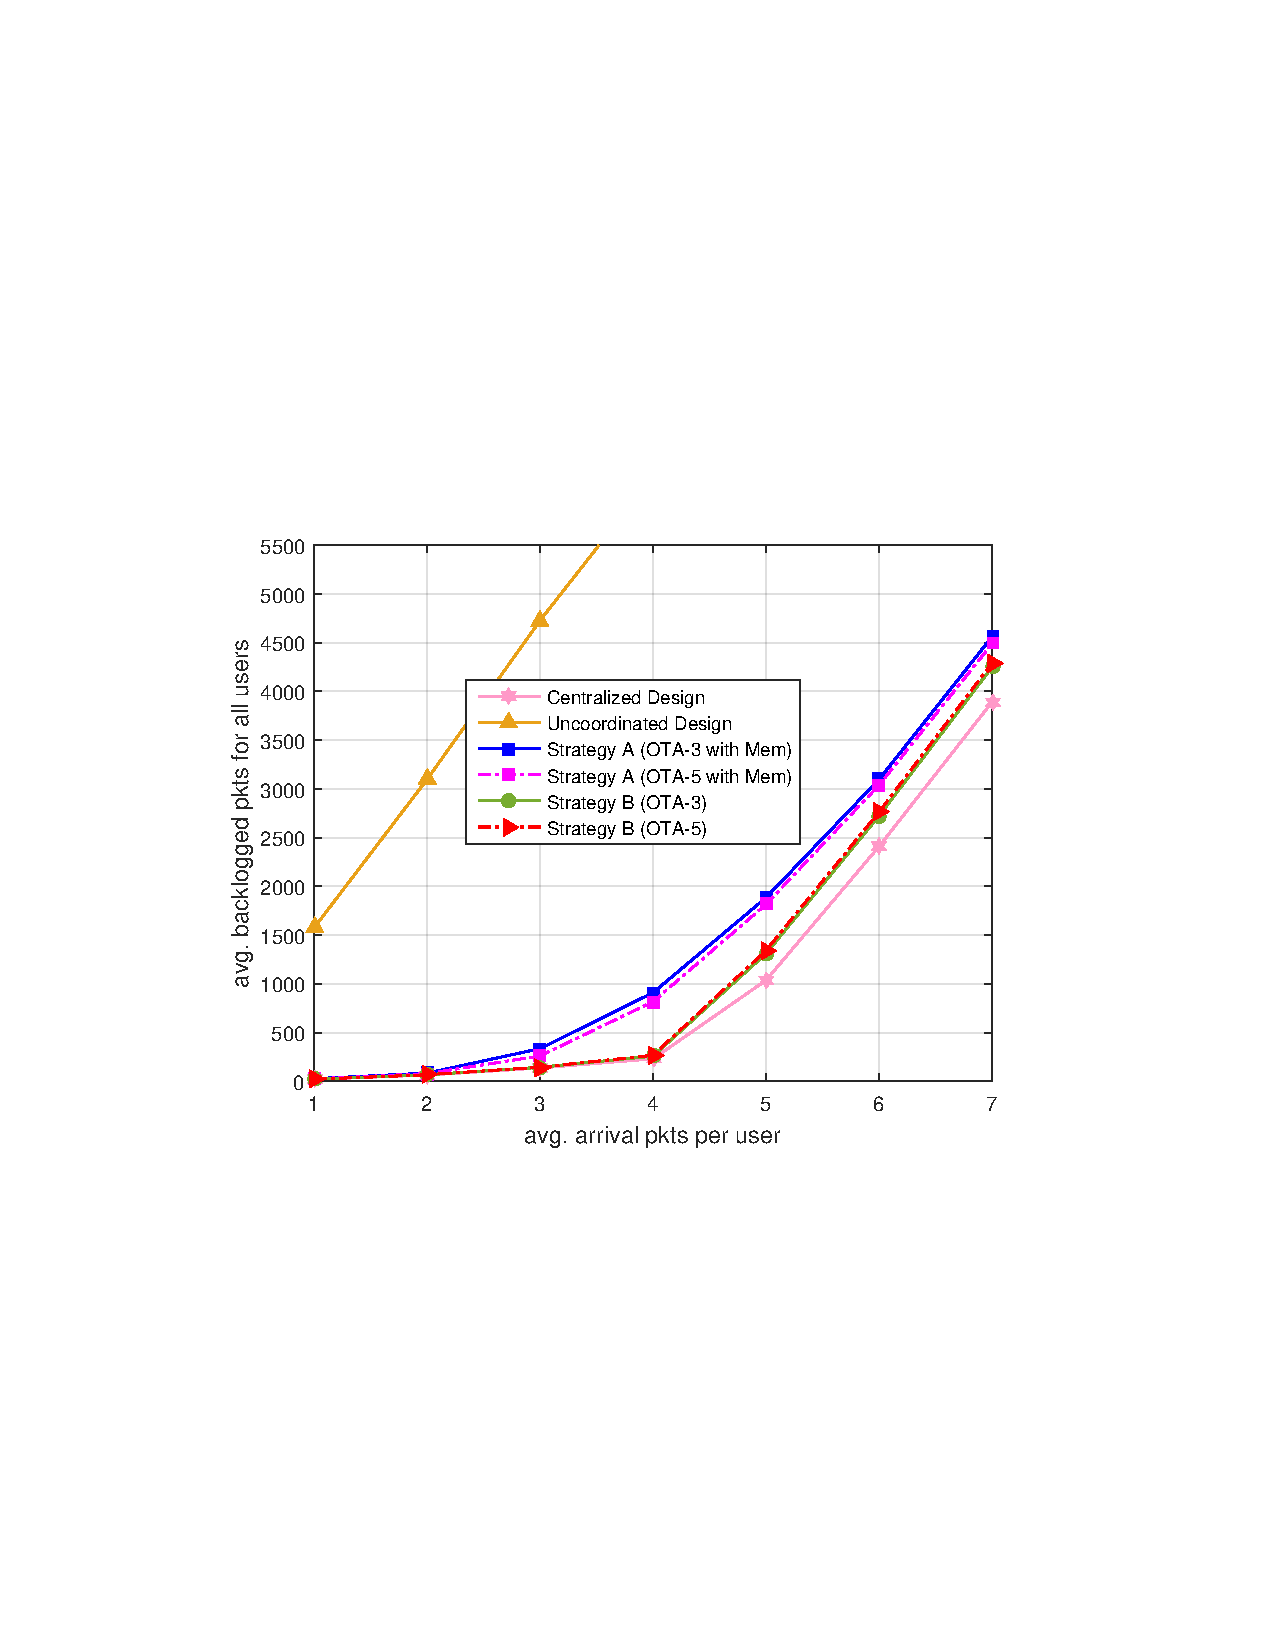
\includegraphics[trim=5mm 90mm 5mm 90mm,clip, width=\columnwidth]{ICC-A-B1}
		\caption{Average backlogged packets for \eqn{\lbrace N,N_B,K,N_T,N_R \rbrace = \lbrace 3,2,12,4,2 \rbrace} evaluated over \eqn{250} slots with \eqn{f_dT_s\approx 0.01}}
		\label{fig-2}
	\end{figure}
\end{frame}




%\begin{frame}{Time Correlated Fading Performance}
%	\begin{figure}
%		\centering
%		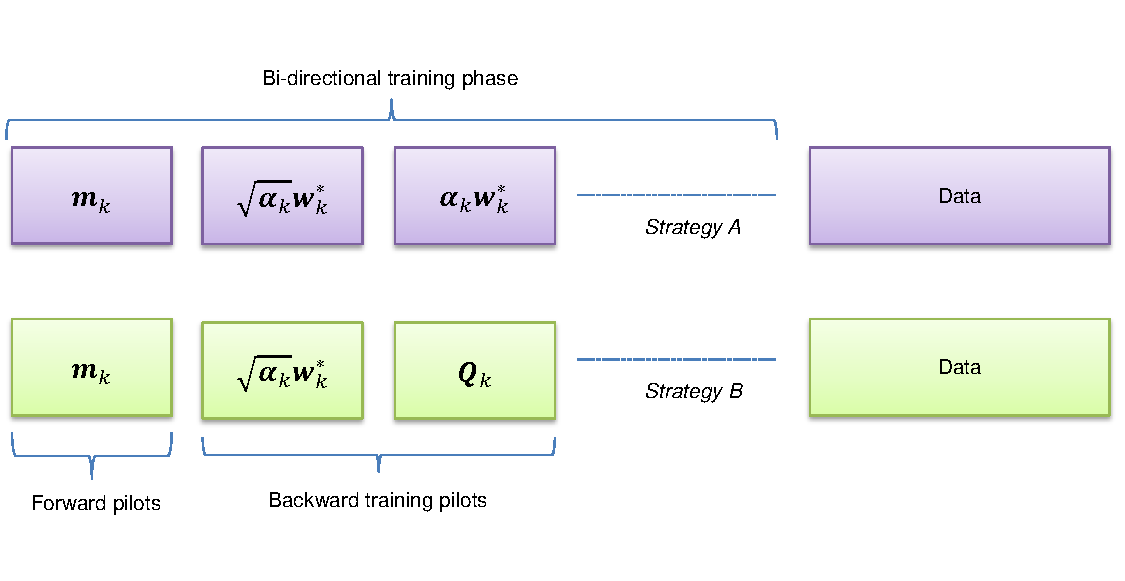
\includegraphics[width=0.75\textwidth]{Doc2}
%		\caption{System Model - \me{\lbrace N,N_B,K,N_R \rbrace = \lbrace 3,2,8,1 \rbrace} after \eqn{250} transmissions}
%	\end{figure}
%\end{frame}
%
%\begin{frame}{Time Correlated Fading Performance}
%\begin{figure}
%	\centering
%	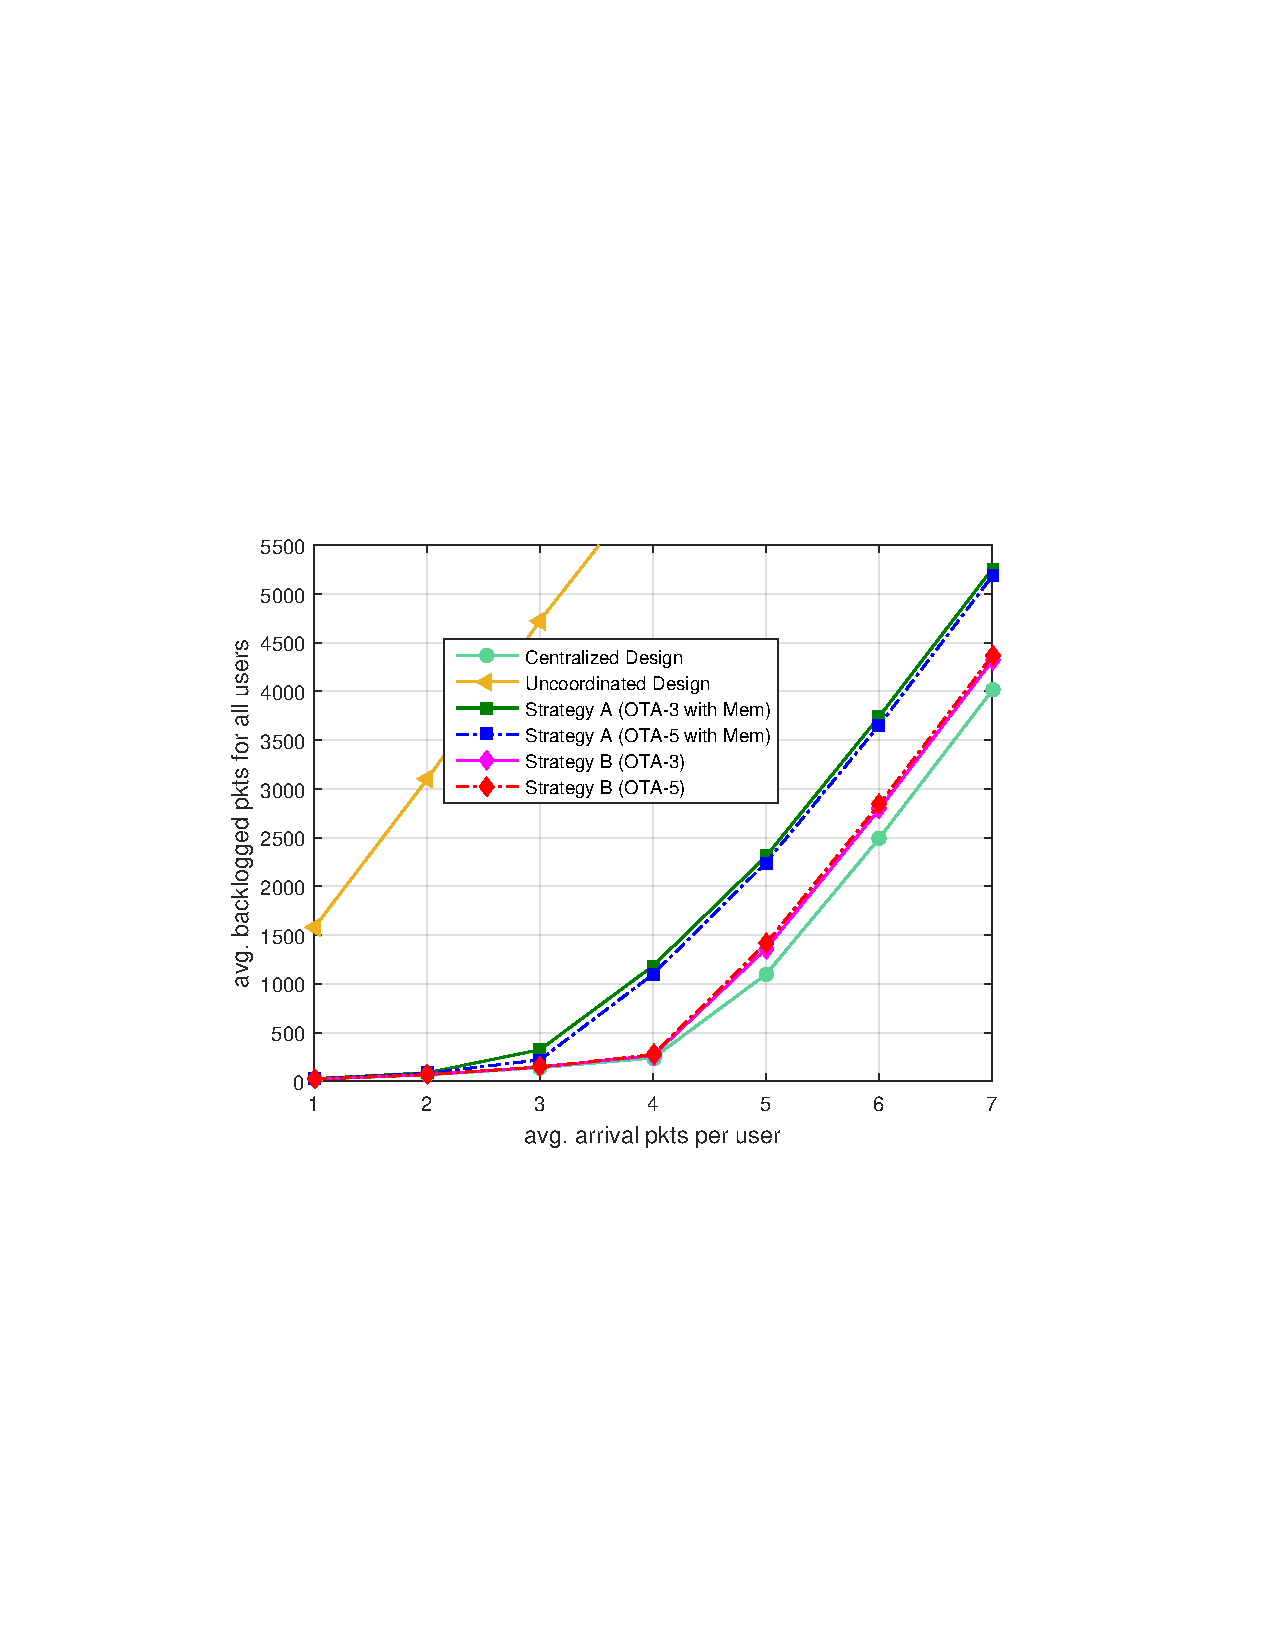
\includegraphics[width=\columnwidth]{ICC-A-B-1}
%	\caption{Average backlogged packets for \eqn{\lbrace N,N_B,K,N_T,N_R \rbrace = \lbrace 3,2,12,4,2 \rbrace} evaluated over \eqn{250} slots with \eqn{f_dT_s\approx 0.1}}
%	\label{fig-1}
%\end{figure}
%\end{frame}


\section{Conclusions}

\begin{frame}{Conclusions}
\begin{itemize}
\item We studied cross layer problem of designing transmit and receive beamformers based on the number of residual packets
\item Since the problem is nonconvex, we solve the problem iteratively by solving convex subproblems in each iteration
\item We also proposed a practical way of implementing the precoder design in a distributed manner by solving the \ac{KKT} expressions
\item Extensions of the proposed work in time-correlated fading scenario with limited number of information exchange cycle is also presented
\end{itemize}
\end{frame}


\begin{frame}
\begin{center}
{\color{blue}\Huge{Questions !}}
\end{center}
\end{frame}

\end{document}
